\documentclass{bmvc2k}

%% Enter your paper number here for the review copy
% \bmvcreviewcopy{??}

\title{CVGlobal}

% Enter the paper's authors in order
\addauthor{Leonardo Ruso}{leonardo.russo@inria.fr}{1}
\addauthor{Diego Marcos}{diego.marcos@inria.fr}{1}

% Enter the institutions
% \addinstitution{Name\\Address}
\addinstitution{
 INRIA\\
 Evergreen Team\\
 Montpellier, France
}

\runninghead{Russo, Marcos}{CVGlobal}

% Any macro definitions you would like to include
% These are not defined in the style file, because they don't begin
% with \bmva, so they might conflict with the user's own macros.
% The \bmvaOneDot macro adds a full stop unless there is one in the
% text already.
\def\eg{\emph{e.g}\bmvaOneDot}
\def\Eg{\emph{E.g}\bmvaOneDot}
\def\etal{\emph{et al}\bmvaOneDot}

%------------------------------------------------------------------------- 
% Document starts here
\begin{document}

\maketitle

\begin{abstract}
Cross-view geo-localization and orientation estimation require models that generalize across diverse geographies. Existing evaluations are often geographically narrow, limiting conclusions about robustness and fairness. We address this by introducing CVGlobal, a geographically balanced test benchmark spanning five continents with paired aerial and street-view imagery across urban and rural contexts. CVGlobal enables geographically fair assessment and facilitates analysis of region-specific behavior.

Alongside the benchmark, we present a training-free, zero-shot baseline for cross-view orientation estimation built on vision foundation models. The method aggregates tokens along vertical (ground) and radial (aerial) directions and incorporates lightweight geometric priors (sky masking and depth cues) to encourage alignment without task-specific training. We evaluate on CVUSA and analyze results on CVGlobal. While the zero-shot baseline underperforms supervised methods in absolute accuracy, it provides meaningful signals, transparent failure modes, and a portable, low-cost reference for ablations and diagnostics.

Our study surfaces generalization gaps across regions and highlights opportunities to combine strong priors with light supervision. We release CVGlobal to catalyze geographically fair evaluation and provide a simple zero-shot baseline to serve as a reproducible yardstick for future supervised and semi-supervised approaches.
\end{abstract}

%------------------------------------------------------------------------- 
\section{Introduction}
\label{sec:intro}

Cross-view geo-localization and orientation estimation underpin applications in robotics, mapping, and outdoor AR, where systems must align ground-view observations with overhead imagery across diverse environments. Despite rapid progress, most evaluations remain geographically narrow (e.g., US-centric), raising concerns about generalization and fairness. We argue that advancing the field requires both: (i) geographically balanced benchmarks, and (ii) strong, training-light baselines that are easy to transfer and diagnose.

This work addresses both needs. First, we introduce CVGlobal, a globally balanced test benchmark spanning five continents with urban and rural regions. CVGlobal enables geographically fair assessment by design, reducing the risk that methods overfit to a single region's visual biases. Second, we present a simple zero-shot baseline for orientation estimation that exploits vision foundation models. Our method aggregates tokens along vertical (ground) and radial (aerial) directions, and uses lightweight geometric priors (sky masking and depth cues) to encourage alignment—all without task-specific training. While zero-shot performance lags supervised methods in absolute accuracy, it provides a transparent, portable reference that helps stress-test assumptions and diagnose failure modes across regions.

We evaluate on CVUSA and report qualitative and quantitative analyses, then use CVGlobal to highlight geographic effects and characterize strengths and limitations of zero-shot orientation estimation. We find that the baseline produces meaningful signals in many scenes and offers a cost-effective yardstick for ablations and future improvements.

Our contributions are:

\begin{itemize}
    \item CVGlobal: a geographically balanced cross-view test benchmark covering five continents with paired aerial and street-view imagery across urban and rural contexts, enabling fairer evaluation and analysis.
    \item A training-free, zero-shot baseline for cross-view orientation estimation built on ViT features, with interpretable vertical/radial token aggregation and simple geometric priors (sky and depth).
    \item An empirical study across CVUSA and CVGlobal that surfaces generalization gaps, clarifies when zero-shot signals are reliable, and establishes a portable baseline for future supervised or semi-supervised methods.
\end{itemize}

\section{Related Works}
\label{sec:related_works}

Cross-view geo-localization addresses the fundamental challenge of matching images captured from drastically different viewpoints of the same geographic location. This task has evolved from traditional handcrafted approaches to sophisticated deep learning methods, driven by applications in augmented reality, robotics, among many other fields.

\subsection{Cross-View Geo-localization and Orientation Estimation}

Early pioneering works by Workman and Jacobs~\cite{workman2015predicting,workman2015learning} established the foundation for cross-view matching by demonstrating the potential of CNNs for learning feature representations across viewpoint variations. The introduction of benchmark datasets like CVUSA~\cite{workman2015predicting} and later VIGOR~\cite{zhu2021vigor} catalyzed systematic research in this domain, with the latter providing more challenging same-area and cross-area evaluation protocols which better reflect real-world deployment scenarios.

Subsequent developments focused on addressing the inherent domain gap between aerial and ground imagery. Notable approaches include CVM-Net~\cite{hu2018cvm}, which introduced dual-stream CNN architectures with polar transformations to align spatial layouts, and SAFA~\cite{NEURIPS2019_ba2f0015}, which employed attention mechanisms for spatial-aware feature aggregation. Methods like CVFT~\cite{shi2019optimalfeaturetransportcrossview} tackled the domain gap through feature transport modules, while others explored generative approaches to synthesize cross-view correspondences~\cite{regmi2018cross}.

The recognition that orientation estimation is crucial for disambiguation and practical applications led to joint location and orientation frameworks. Recent works have emphasized the importance of spatial awareness in feature representations~\cite{shi2020ilookingatjoint}, particularly for applications requiring precise alignment such as outdoor augmented reality. However, many existing methods either treat orientation as a byproduct of location retrieval or require extensive supervised training with orientation labels.

The advent of Vision Transformers (ViTs)~\cite{dosovitskiy2020image} has revolutionized the whole computer vision field by enabling models to capture global spatial relationships through self-attention mechanisms. Transformer-based approaches like L2LTR~\cite{yang2021cross} and TransGeo~\cite{wang2021multi} have demonstrated superior performance over CNN-based methods, leveraging learnable position encodings and global context modeling.

Concurrently, self-supervised learning has emerged as a powerful paradigm for learning visual representations without manual annotations. Methods such as MoCo~\cite{he2020momentum}, SimCLR~\cite{chen2020simple}, and BYOL~\cite{grill2020bootstrap} have shown that self-supervised features can match or exceed supervised counterparts on various downstream tasks. DINOv2~\cite{oquab2023dinov2} represents the current state-of-the-art for visual transformers, providing features particularly well-suited for dense prediction tasks and fine-grained visual understanding.

Despite these advances, most transformer-based cross-view methods still rely heavily on supervised learning with orientation labels, requiring extensive annotation efforts. Recent works have begun exploring self-supervised features for geo-localization tasks, but typically treat cross-view matching as standard retrieval without considering the specific geometric constraints and orientation relationships inherent in cross-view scenarios.

% Recent research has recognized the value of incorporating complementary modalities to improve cross-view matching performance. Sky segmentation techniques help eliminate uninformative regions in ground-level images, focusing attention on building structures and terrain features visible in aerial views~\cite{workman2015predicting}. Advanced monocular depth estimation models like Depth-Anything~\cite{yang2024depth} provide robust geometric cues that enable multi-scale feature aggregation and informed spatial reasoning.

% Attention mechanisms have proven particularly effective for cross-view alignment, with cross-attention layers learning to focus on corresponding regions between aerial and ground views. However, most attention-based methods require supervised training with orientation labels and struggle with the limited field-of-view constraints common in real-world applications.

\subsection{Cross-Modality Datasets}

Current benchmark datasets, while valuable, present limitations for comprehensive evaluation. CVUSA focuses primarily on the United States, while VIGOR, though more diverse, still covers a limited geographical scope. These datasets primarily support geo-localization and retrieval tasks, with growing interest in orientation estimation as a distinct but related problem. The lack of large-scale, geographically diverse datasets with comprehensive global coverage has hindered the development of truly robust cross-view methods that generalize across different environmental conditions and cultural contexts.

Our work addresses these limitations by introducing CVGlobal, a large-scale dataset with balanced global representation, and proposing a novel cross-view method that combines unsupervised features with multi-modal cues for orientation estimation.

\section{Dataset Generation Method}
\label{sec:dataset_generation}

In this section, we present our methodology for constructing CVGlobal, a multi-modal dataset that pairs satellite and street-view imagery across diverse global regions. Our approach systematically samples locations from five continents while ensuring geographical diversity and balanced representation between urban and rural environments.

\subsection{Dataset Design and Sampling Strategy}

Our dataset construction methodology is guided by two key principles: \textit{geographical diversity} and \textit{balanced representation}. We define sampling regions across five major continents (North America, Europe, Asia, South America, and Africa), with each continent contributing equally to the final dataset to prevent geographical bias.

For each continent, we establish two distinct sampling regions:
\begin{itemize}
    \item \textbf{Urban regions}: Areas with high population density and significant urban infrastructure
    \item \textbf{Rural regions}: Areas with low population density and predominantly natural or agricultural landscapes
\end{itemize}

The sampling regions are carefully selected to represent diverse climatic, cultural, and developmental contexts within each continent. Table~\ref{tab:sampling_regions} details the specific geographical boundaries for each region.

\begin{table}[t]
\centering
\caption{Geographical sampling regions defined for each continent and environment type.}
\label{tab:sampling_regions}
\begin{tabular}{lllcc}
\toprule
\textbf{Continent} & \textbf{Type} & \textbf{Location} & \textbf{Lat Range} & \textbf{Lon Range} \\
\midrule
North America & Urban & New York City & 40.71°--40.81°N & 74.01°--73.91°W \\
              & Rural & California Farmland & 36.78°--36.88°N & 119.42°--119.32°W \\
\midrule
Europe & Urban & Paris & 48.86°--48.96°N & 2.35°--2.45°E \\
       & Rural & French Countryside & 46.23°--46.33°N & 2.21°--2.31°E \\
\midrule
Asia & Urban & Tokyo & 35.69°--35.79°N & 139.69°--139.79°E \\
     & Rural & Rural India (Agra) & 27.18°--27.28°N & 78.04°--78.14°E \\
\midrule
South America & Urban & São Paulo & 23.55°--23.45°S & 46.63°--46.53°W \\
              & Rural & Brazilian Rainforest & 14.24°--14.13°S & 51.93°--51.83°W \\
\midrule
Africa & Urban & Nairobi & 1.29°--1.19°S & 36.82°--36.92°E \\
       & Rural & Kenyan Savanna & 2.15°--2.05°S & 37.31°--37.41°E \\
\bottomrule
\end{tabular}
\end{table}

% add the image
\begin{figure}[t]
    \centering
    \includegraphics[width=0.9\linewidth]{images/sampling_regions_map.png}
    \caption{Global distribution of CVGlobal dataset sampling regions across five continents, showing urban (red) and rural (teal) areas with numbered locations corresponding to Table~\ref{tab:sampling_regions}.}
    \label{fig:sampling_regions}
\end{figure}

\subsection{Data Acquisition Details}

The CVGlobal dataset has been generated ensuring high-quality multi-modal data collection through random coordinate sampling. For each region, we generate random coordinates and validate them for Street View availability and outdoor environments using Google Places API filtering to exclude indoor locations such as shopping malls and restaurants.

For each validated coordinate, we acquire satellite imagery (640×640 pixels at zoom level 18) and street-view images from four cardinal directions (0°, 90°, 180°, 270°). The directional images are concatenated to create panoramic representations.

\section{Crossview Method}
\label{sec:method}

\begin{figure}[t]
    \centering
    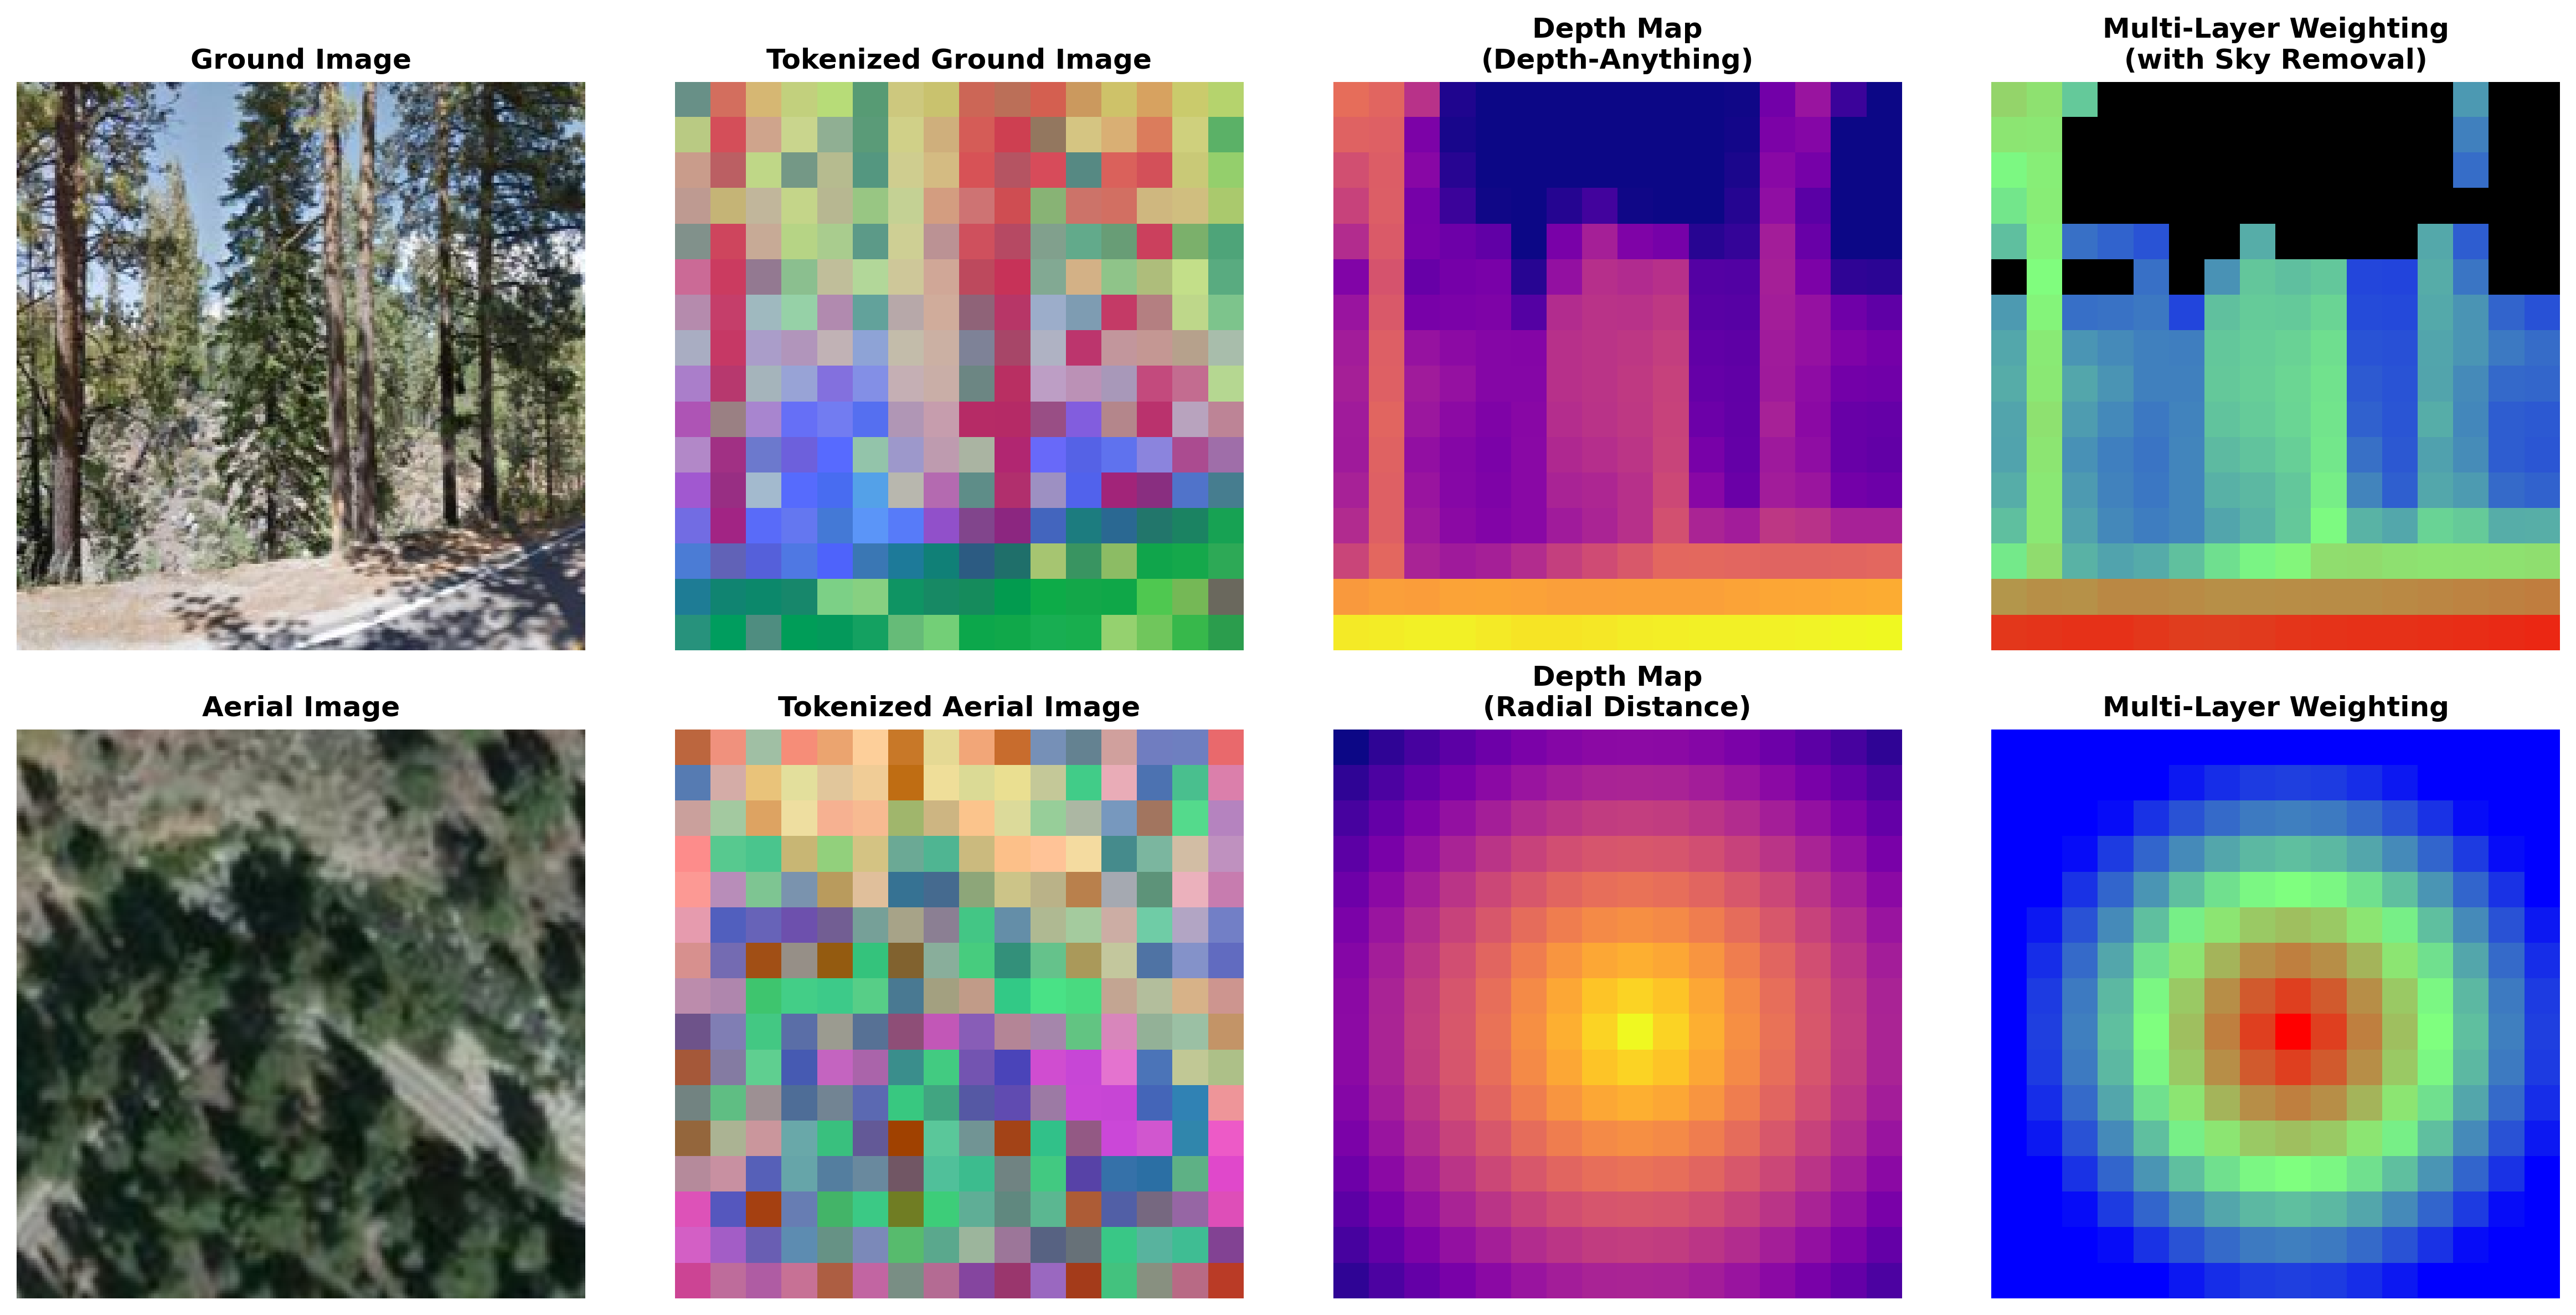
\includegraphics[width=0.9\linewidth]{images/tokenized_depth_visualization.png}
    \caption{Visualization of tokenized depth information for aerial images, highlighting the spatial distribution of depth cues across different regions.}
    \label{fig:method}
\end{figure}

We propose PROJECT\_NAME, a novel approach for cross-view orientation estimation that leverages a ViT backbne for feature extraction with orientation-aware token aggregation strategies. Our method addresses the fundamental challenge of aligning ground-level images with aerial satellite views by exploiting both spatial structure and depth information through a flexible architecture that supports multiple vision foundation models.

\subsection{Problem Formulation}

Given a ground-level panoramic image $I_g$ and an aerial satellite image $I_a$ of the same geographic location, our goal is to estimate the relative orientation $\theta$ between the two views. The ground image is extracted from a 360° panorama using a field-of-view (FOV) window defined by parameters $(f_x, f_y, \psi, \phi)$, where $f_x$ and $f_y$ represent the horizontal and vertical FOV angles, $\psi$ is the yaw (rotation around the vertical axis), and $\phi$ is the pitch (elevation angle).

\subsection{Feature Extraction}

PROJECT\_NAME employs a flexible architecture that can utilize different pre-trained ViT models as feature extractors. Our implementation supports multiple backbone architectures including DINOv2 and CLIP.

The feature extraction process is consistent for any backbone model used, and it will be treated as a black box for the scope of this work.

\begin{align}
\mathbf{T}_g &= \text{Backbone}(I_g) \\
\mathbf{T}_a &= \text{Backbone}(I_a) 
\end{align}

where $\mathbf{T}_g$, $\mathbf{T}_g \in \mathbb{R}^{(G, G, C)}$ are the ground and aerial tokens respectively, where $G$ represents the grid size, and $C$ represents the number of channels for each token. Their size changes on the backbone model used, depending on its patch size:

\begin{itemize}
    \item \textbf{DINOv2} uses the pre-trained DINOv2-ViT-B/14 model with 14×14 pixel patches, producing a $16 \times 16$ token grid with 768-dimensional features.
    \item \textbf{CLIP} employs CLIP-ViT-Base-Patch16 with 16×16 pixel patches, generating a $14 \times 14$ token grid with 768-dimensional features.
\end{itemize}

\subsection{Sky Filtering and Depth Estimation}

To improve orientation estimation, we incorporate the following semantic and geometric priors to the ground and aerial images:

\textbf{Sky Segmentation}: We employ a lightweight CNN-based sky filter to identify and mask sky regions in ground images. The sky mask $M_{sky}$ is computed at the patch level using majority voting within each grid cell, producing a binary mask $M_{grid} \in \{0,1\}^{G \times G}$ where 1 indicates ground and 0 indicates sky.

\textbf{Depth Estimation}: For ground imagery, we utilize the Depth-Anything model to generate depth maps $D^{(G)}_{grid}$ for each image. The depth information is downsampled to match the token grid, providing normalized depth values $d_{i,j} \in [0,1]$ for each spatial location $(i,j)$.

For aerial imagery instead, we create a comparative depth map by using the radial distance from the center of the image to each pixel. Subsequently, the pixel values are averaged to compute the depth map $D^{(A)}_{grid}$ at the patch level.

\subsection{Multi-Layer Depth-Weighted Token Aggregation}

We introduce a novel aggregation strategy that separates tokens into three depth layers: \textit{foreground, middleground, and background}. This approach captures the multi-scale nature of visual features in cross-view matching.

\textbf{Vertical Column Analysis}: For each vertical column $j$ in the ground image feature grid, we compute depth-weighted averages over valid (non-sky) tokens:

\begin{align}
\mathbf{t}_j^{fore} &= \frac{\sum_{i: M_{grid}(i,j)=1} w_i^{fore} \cdot \mathbf{f}_{i,j}^g}{\sum_{i: M_{grid}(i,j)=1} w_i^{fore}} \\
\mathbf{t}_j^{mid} &= \frac{\sum_{i: M_{grid}(i,j)=1} w_i^{mid} \cdot \mathbf{f}_{i,j}^g}{\sum_{i: M_{grid}(i,j)=1} w_i^{mid}} \\
\mathbf{t}_j^{back} &= \frac{\sum_{i: M_{grid}(i,j)=1} w_i^{back} \cdot \mathbf{f}_{i,j}^g}{\sum_{i: M_{grid}(i,j)=1} w_i^{back}}
\end{align}

where the depth-dependent weights are defined as:
\begin{align}
w_i^{fore} &= d_{i,j} \\
w_i^{mid} &= \begin{cases} 
\frac{d_{i,j}}{\tau} & \text{if } d_{i,j} \leq 0.5 \\
\frac{1-d_{i,j}}{d_{i,j}} & \text{otherwise}
\end{cases} \\
w_i^{back} &= 1 - d_{i,j}
\end{align}

with threshold $\tau = 0.5$. This weighting scheme emphasizes close objects for foreground, balanced weights for middleground, and distant objects for background layers.

\textbf{Radial Direction Analysis}: For aerial images, we extract features along radial directions from the center, using linear weight progressions:

\begin{align}
\mathbf{r}_\beta^{fore} &= \frac{\sum_{r=0}^{R} w_r^{fore} \cdot \mathbf{f}_{\beta,r}^a}{\sum_{r=0}^{R} w_r^{fore}} \\
\mathbf{r}_\beta^{mid} &= \frac{\sum_{r=0}^{R} w_r^{mid} \cdot \mathbf{f}_{\beta,r}^a}{\sum_{r=0}^{R} w_r^{mid}} \\
\mathbf{r}_\beta^{back} &= \frac{\sum_{r=0}^{R} w_r^{back} \cdot \mathbf{f}_{\beta,r}^a}{\sum_{r=0}^{R} w_r^{back}}
\end{align}

where $\beta$ represents the angular direction, $r$ is the radial distance from center, and the weights follow: $w_r^{fore} = 1-r/R$ (decreasing), $w_r^{back} = r/R$ (increasing), and $w_r^{mid}$ follows a triangular pattern peaking at the center.

\subsection{Cross-Modal Orientation Estimation}

\begin{figure}[t]
    \centering
    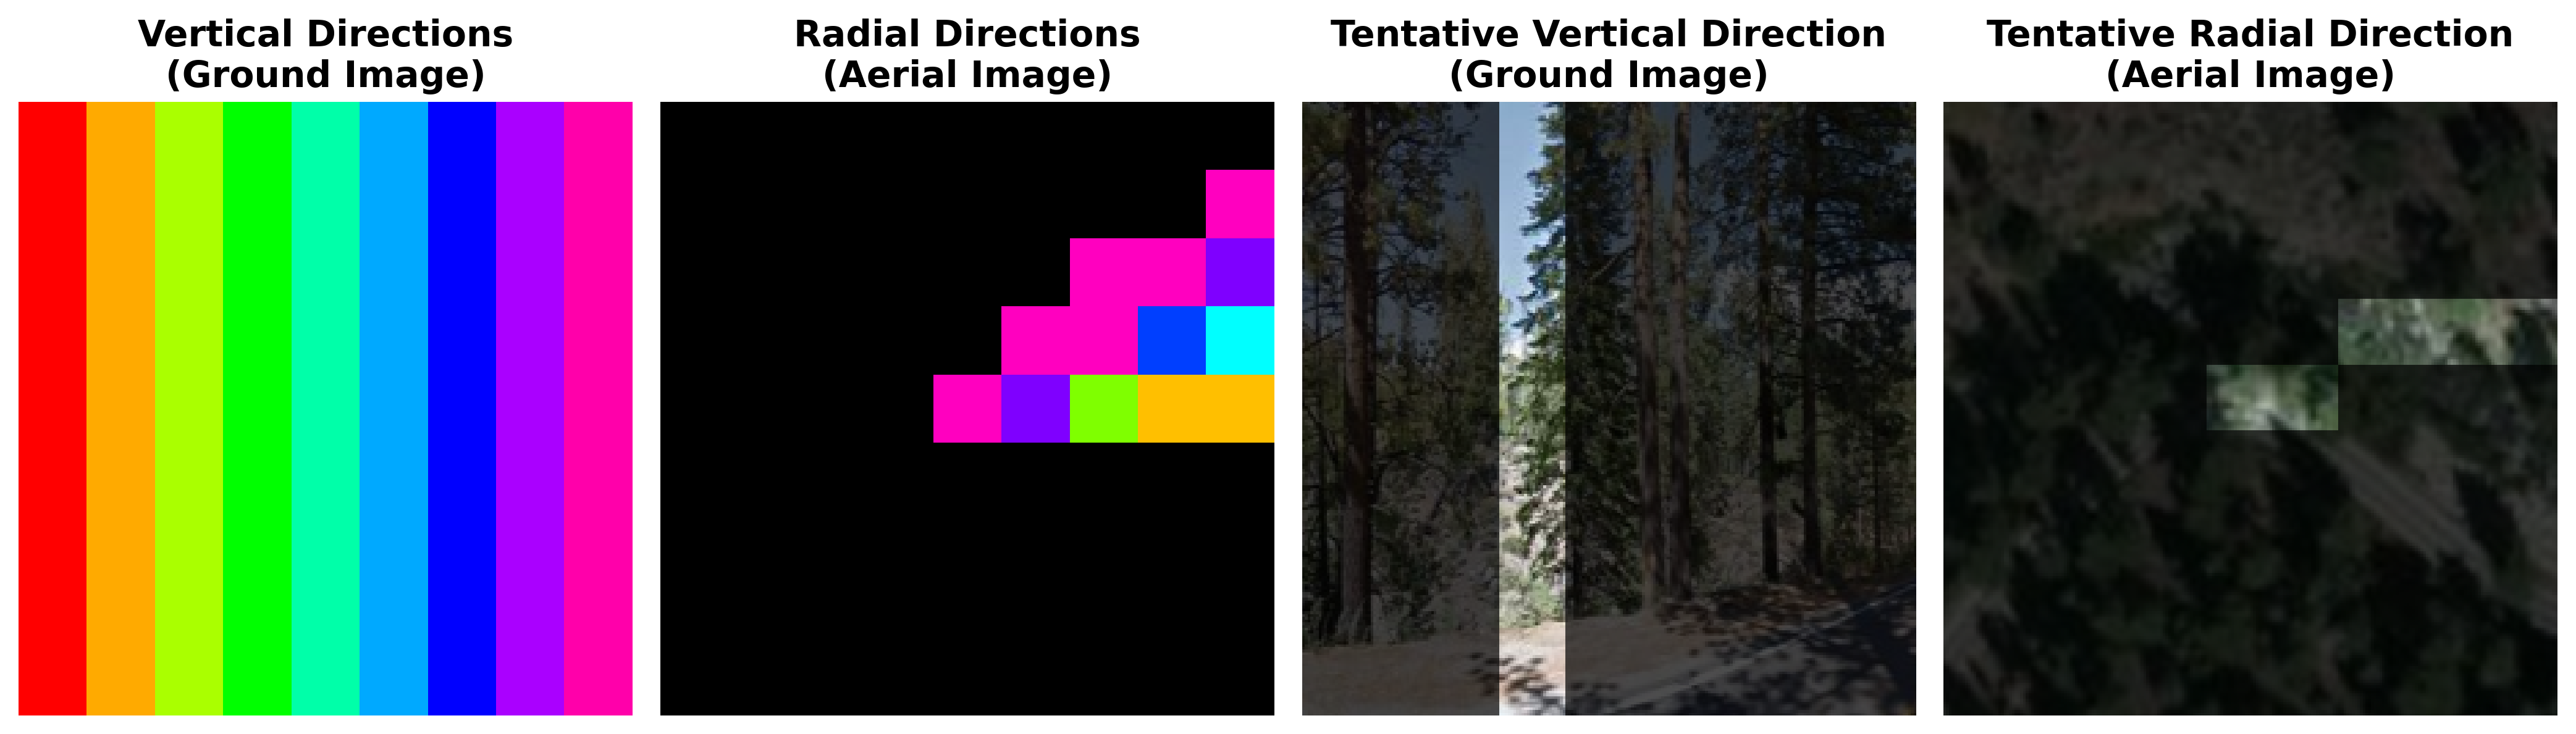
\includegraphics[width=0.9\linewidth]{images/rainbow_directions.png}
    \caption{Radial directions used for aerial image token aggregation, visualized as a rainbow pattern. Each color represents a distinct radial direction corresponding to the angular offset from the center of the aerial image.}
    \label{fig:directions}
\end{figure}

We estimate orientation by finding the angular offset that minimizes the cosine distance between corresponding vertical and radial feature aggregations. For each candidate orientation $\theta$, we compute the alignment cost:

\begin{align}
\mathcal{L}(\theta) = \frac{1}{G} \sum_{i=0}^{G} \left\| 1 - \begin{bmatrix} \mathbf{t}_{G-1-i}^{fore} \\ \mathbf{t}_{G-1-i}^{mid} \\ \mathbf{t}_{G-1-i}^{back} \end{bmatrix}^T \begin{bmatrix} \mathbf{r}_{\phi(\theta,i)}^{fore} \\ \mathbf{r}_{\phi(\theta,i)}^{mid} \\ \mathbf{r}_{\phi(\theta,i)}^{back} \end{bmatrix} \right\|
\end{align}

where $\phi(\theta,i) = (\lfloor\theta/\Delta\theta\rfloor + i - G/2) \bmod |\mathcal{R}|$ maps vertical columns to radial directions, $\Delta\theta = \text{FOV}_x / G$ is the angular step size.

The optimal orientation is then found as:
\begin{align}
\theta^* = \arg\min_{\theta \in [0, 2\pi)} \mathcal{L}(\theta)
\end{align}

To assess the reliability of orientation estimates, we compute a confidence score based on the Z-score of the minimum distance:

\begin{align}
\text{confidence} = \frac{\mu(\mathcal{L}) - \min(\mathcal{L})}{\sigma(\mathcal{L})}
\end{align}

where $\mu(\mathcal{L})$ and $\sigma(\mathcal{L})$ are the mean and standard deviation of the loss values across all candidate orientations. Higher confidence scores indicate more reliable orientation estimates.

\section{Results}

To evaluate the performance of the proposed method, we analyze its performance in the CVUSA dataset and we compare our method against state-of-the-art approaches in cross-view orientation estimation. 

The CVUSA dataset includes panoramic images, from which we extract random FOV windows with:

\begin{table}[H]
\centering
\begin{tabular}{c|c}
FOV$_x$ & $90^\circ$ \\
\hline
FOV$_y$ & $180^\circ$ \\
\hline
Yaw & $\psi \sim (0^\circ, 360^\circ)$ \\
\end{tabular}
\caption{FOV and yaw settings for the CVUSA dataset.}
\label{tab:cvusa_fov_yaw}
\end{table}

Aerial images undergo center cropping and resizing to match the standard $224\times224$ ViT input size.

Then, we apply our method to all the images belonging to the CVPR subset of CVUSA, storing the errors in orientation estimates for evaluation.

\begin{figure}[H]
    \centering
    \includegraphics[width=0.9\linewidth]{images/grid_4x4.png}
    \caption{Orientation estimation errors for the CVPR subset of CVUSA dataset. Each bar represents the average error for a specific image, highlighting the effectiveness of our method in various scenarios.}
    \label{fig:orientation_errors}
\end{figure}



\section{Conclusions}
\label{sec:conclusions}

We presented a zero-shot approach to cross-view orientation estimation that leverages strong vision foundation models with simple, interpretable token-aggregation and lightweight geometric priors (sky filtering and depth cues). While our experiments show that this zero-shot pipeline underperforms supervised counterparts in absolute accuracy, it offers several positives: no task-specific training, easy portability across backbones, transparent failure modes, and a low-cost baseline for rapid analysis and ablations. In practice, we find it provides meaningful signals in many scenes and can serve as a diagnostic tool or complementary component within stronger systems.

Beyond the method, this work contributes a new test benchmark with balanced global coverage. The CVGlobal evaluation set spans diverse continents and urban/rural contexts, enabling geographically fair assessment and reducing region-specific bias. We hope this resource will facilitate more rigorous comparisons and catalyze progress toward globally robust cross-view localization and orientation estimation.

Future work includes integrating light supervision to bridge the zero-shot gap, exploring improved geometric priors and uncertainty calibration, and scaling evaluation across additional modalities.

\bibliography{egbib}
\end{document}
